\documentclass{article}
\usepackage[preprint]{neurips_2026}
\usepackage[T1]{fontenc}
\usepackage[utf8]{inputenc}
\usepackage{amsmath,amssymb,booktabs}
\usepackage{graphicx,pgfplots,placeins}
\usepackage[hidelinks]{hyperref}
\pgfplotsset{compat=1.18,every axis/.append style={font=\small,grid=major,grid style={gray!15},tick label style={font=\footnotesize},label style={font=\small}}}
\definecolor{polyured}{RGB}{165,28,48}
\title{Convex Optimization for Sparse Signal Reconstruction\\A Comparative Study of ISTA, FISTA and ADMM}
\author{Group 3\thanks{Code, data and reproduction instructions: \url{https://github.com/DongkuanWu/COMP6704-Group3-LASSO}.}\\COMP6704\\The Hong Kong Polytechnic University}
\begin{document}
\raggedbottom
\maketitle
\begin{abstract}
We compare ISTA, FISTA and ADMM on a shared LASSO benchmark comprising ten settings, twenty independent instances per setting and five timing repeats per solver. All 3,000 runs reached their specified stopping thresholds, with a maximum within-instance spread of $2.30\times10^{-6}$ in the final objective values. At baseline, ADMM required 40.5 updates on average, compared with 95 for FISTA and 148 for ISTA, but matrix preparation dominated its elapsed time. FISTA averaged 1.74 ms and ISTA 2.12 ms. FISTA had lower mean time in nine of ten settings. Recovery error depended strongly on the available measurements and regularization strength. These experiments show why objective accuracy, recovery quality and elapsed time must be examined together. The conclusions describe the tested dense implementations and synthetic data distribution.
\end{abstract}

\section{Introduction}
Sparse signal reconstruction addresses an information constraint that occurs when a measurement system records fewer observations than the number of unknown coefficients. Each row of a sensing matrix describes one linear measurement. When the number of measurements is smaller than the signal dimension, the observations leave a nontrivial set of candidate signals. Sparsity narrows that set by specifying that most coefficients are zero. In the baseline experiment considered here, 96 measurements describe 192 coefficients, with ten active entries. The reconstruction procedure must infer both the active locations and their amplitudes from the observed mixtures.

The distinction between fitting and identification is central to this problem. For any vector in the null space of the measurement matrix, adding that vector to a candidate signal leaves its predicted measurements unchanged. A data-fitting criterion alone therefore cannot select a unique signal in the underdetermined setting. Noise adds a second difficulty: exact agreement with the observations can also reproduce the noise. A reconstruction model must combine measurement consistency with a structural preference that reflects the signal class.

The LASSO formulation supplies this combination through a squared residual and an $\ell_1$ penalty. The residual penalizes disagreement with the observations, while the penalty promotes coefficient shrinkage and exact zeros through the proximal update. Both terms are convex. Consequently, the model supports algorithms whose updates can be evaluated against a common optimality criterion. At the same time, the regularized solution is influenced by the penalty parameter. Driving an optimization residual to a small value establishes numerical accuracy for the chosen objective, while recovering the physical signal also depends on the observations and regularization bias.

ISTA, FISTA and ADMM offer three distinct computational routes to this shared objective. ISTA repeatedly applies a gradient update followed by soft thresholding. FISTA adds extrapolation to the same proximal step. ADMM splits the fitting and sparsity terms into coupled subproblems and introduces a linear-system preparation cost. These differences produce a practical evaluation problem: one iteration does not represent the same amount of work across solvers. A method that reduces update counts can still require more elapsed time when its preparation or per-step cost is larger.

We therefore evaluate the methods at four levels. Objective values establish numerical agreement on the optimization task. Relative signal error measures reconstruction quality against the known synthetic truth. Iteration counts characterize progress per update. Measured time captures the cost of the specific implementation, including its recorded setup operations. The experiments pair solvers on the same instances and summarize repeated timings before statistical comparisons. This design connects algorithmic behavior to observed execution cost without treating five measurements of one instance as five independent signals.

The study makes three empirical contributions. First, it compares the three methods over ten controlled configurations and 200 problem instances, with 3,000 timed runs. Second, it decomposes ADMM time and measures within-instance timing variation, exposing the implementation and measurement effects behind the elapsed-time results. Third, it examines how measurement count, sparsity, noise and regularization alter recovery quality after convergence. The resulting analysis identifies precisely which rankings hold in the archived benchmark and which experimental changes are needed to test additional explanations.


\paragraph{Connection to sparse estimation.}
LASSO was introduced as a method for simultaneous shrinkage and variable selection \citep{tibshirani1996}. Here its coefficients represent a synthetic sparse signal rather than predictors selected from an observational dataset. The same squared-loss model links these interpretations, but recovery of the true support requires assumptions on the sensing matrix, noise and signal amplitudes. Sparsity alone does not guarantee identifiability. Proximal methods exploit the separability of the penalty \citep{parikh2014}, while the split formulation of ADMM separates the fitting and shrinkage operations. Our comparison studies these computational choices at fixed problem instances.

\section{Methodology}
\subsection{Observation model and objective}
Let $A\in\mathbb{R}^{m\times n}$ be a known measurement matrix, $x^\star\in\mathbb{R}^n$ an unknown signal, and $\varepsilon\in\mathbb{R}^m$ additive noise. The input observations satisfy
\begin{equation}
 b=Ax^\star+\varepsilon,\qquad m<n,\qquad \|x^\star\|_0=s.
\end{equation}
Since $A$ has a nontrivial null space, fitting the observations alone generally leaves multiple candidate solutions. We estimate the signal by solving
\begin{equation}\label{eq:lasso}
 \min_{x\in\mathbb{R}^n}F(x)=\underbrace{\tfrac12\|Ax-b\|_2^2}_{f(x)}+\lambda\|x\|_1,
 \qquad \lambda=\alpha\|A^\top b\|_\infty.
\end{equation}
The first term measures data fidelity. The second encourages sparsity through coefficient shrinkage. Its weight $\lambda>0$ determines the fit--shrinkage trade-off. The Hessian of $f$ is $A^\top A\succeq0$, and the $\ell_1$ norm is convex. Thus every local minimum of~\eqref{eq:lasso} is global, although uniqueness requires additional conditions \citep{boyd2004}.

We distinguish optimization accuracy from reconstruction quality. Objective agreement indicates that solvers reach similar values of $F$. Relative reconstruction error measures the distance to the known synthetic signal,
\begin{equation}
 E(x)=\frac{\|x-x^\star\|_2}{\|x^\star\|_2}.
\end{equation}
Noise and shrinkage bias can leave a nonzero reconstruction error even after the optimization has converged.


\paragraph{Optimality and the critical penalty.}
For $\lambda>0$, the objective is continuous and coercive, so a minimizer exists. Write $\widehat x$ for a minimizer and reserve $x^\star$ for the true signal. Convex optimality is equivalent to
\begin{equation}
0\in A^\top(A\widehat x-b)+\lambda\partial\|\widehat x\|_1,
\qquad
[A^\top(b-A\widehat x)]_i\in
\begin{cases}
\{\lambda\operatorname{sign}(\widehat x_i)\},&\widehat x_i\ne0,\\
[-\lambda,\lambda],&\widehat x_i=0.
\end{cases}
\end{equation}
Consequently, zero is a minimizer if and only if $\lambda\ge\lambda_{\max}:=\|A^\top b\|_\infty$. Our choice $\lambda=\alpha\lambda_{\max}$ expresses the penalty relative to this threshold. On an active coordinate the residual correlation has magnitude $\lambda$, explaining the shrinkage bias even with noiseless data. Uniqueness is a separate issue: one sufficient condition is full column rank of $A_E$, where $E=\{i:|a_i^\top(b-A\widehat x)|=\lambda\}$ is the equicorrelation set \citep{tibshirani2013}. Full rank of only one solution's active columns is not a general uniqueness certificate.

\subsection{ISTA and FISTA}
The gradient $\nabla f(x)=A^\top(Ax-b)$ has Lipschitz constant $L=\|A\|_2^2$. Define the componentwise soft-thresholding operator
\begin{equation}
 [S_\tau(v)]_i=\operatorname{sign}(v_i)\max\{|v_i|-\tau,0\}.
\end{equation}
ISTA takes a proximal gradient step,
\begin{equation}
 x_{k+1}=S_{\lambda/L}\!\left(x_k-\frac{1}{L}\nabla f(x_k)\right).
\end{equation}
FISTA applies this step at an extrapolated point $y_k$. Starting from $x_0=y_0=0$ and $t_0=1$, its updates are
\begin{align}
 x_{k+1}&=S_{\lambda/L}\!\left(y_k-\frac{1}{L}\nabla f(y_k)\right),\\
 t_{k+1}&=\frac{1+\sqrt{1+4t_k^2}}{2},\qquad
 y_{k+1}=x_{k+1}+\frac{t_k-1}{t_{k+1}}(x_{k+1}-x_k).
\end{align}
Both methods mainly use dense matrix--vector products per iteration. The acceleration mechanism can reduce the number of updates, while adding vector operations at each step \citep{beck2009}. Soft thresholding is the proximal map of the $\ell_1$ penalty.


\paragraph{Why soft thresholding solves the proximal step.}
The bound $\|\nabla f(x)-\nabla f(y)\|_2\le L\|x-y\|_2$ yields
$f(x)\le f(y)+\langle\nabla f(y),x-y\rangle+(L/2)\|x-y\|_2^2$.
Minimizing this upper bound plus $\lambda\|x\|_1$ reduces, coordinate by coordinate, to minimizing
$\frac12(v_i-x_i)^2+(\lambda/L)|x_i|$ with $v=y-\nabla f(y)/L$.
The scalar condition $0\in x_i-v_i+(\lambda/L)\partial|x_i|$ gives $v_i-\lambda/L$ for $v_i>\lambda/L$, $v_i+\lambda/L$ for $v_i<-\lambda/L$, and zero otherwise. This is precisely soft thresholding \citep{parikh2014}.

\paragraph{Descent and convergence rates.}
Let $G_L(x)=L[x-S_{\lambda/L}(x-\nabla f(x)/L)]$. Its zero set is the LASSO solution set. Strong convexity of the quadratic surrogate gives the correct ISTA descent inequality
\begin{equation}
F(x_{k+1})\le F(x_k)-\frac{1}{2L}\|G_L(x_k)\|_2^2.
\end{equation}
Thus the objective is nonincreasing, with strict decrease at a nonstationary iterate in exact arithmetic. For any minimizer $\widehat x$, fixed-step ISTA and FISTA satisfy \citep{beck2009}
\begin{align}
F(x_k^{\rm ISTA})-F(\widehat x)&\le\frac{L\|x_0-\widehat x\|_2^2}{2k},\\
F(x_k^{\rm FISTA})-F(\widehat x)&\le\frac{2L\|x_0-\widehat x\|_2^2}{(k+1)^2}.
\end{align}
These are objective-gap guarantees, not rates for our normalized residual or reconstruction error. FISTA need not decrease the objective at every update. Disabling extrapolation recovers the ISTA update, making ISTA a momentum-free algorithmic control; the recorded timing difference also includes the overhead of the distinct implementations.

\paragraph{Dense implementation cost.}
Computing the exact spectral norm by a dense SVD costs $O(m^2n)$ for $m<n$ and is outside the timers. Each ISTA/FISTA gradient uses $A^\top(Ax)$ without forming the Gram matrix, giving $O(mn)$ work per iteration and $O(mn+n)$ storage. Thresholding and momentum require $O(n)$ vector work. Precomputing $A^\top b$ costs $O(mn)$ and is also outside these two solvers' timers. Residual checks perform additional matrix-vector products at scheduled checkpoints. Therefore the theoretical iteration bounds do not directly specify elapsed-time rankings.

\subsection{ADMM}
% ADMM introduces $z$ with the constraint $x=z$, separating the quadratic loss from the nonsmooth penalty \citep{boyd2011}. With scaled dual variable $u$ and $\rho=1$, the updates are
% \begin{align}
%  x_{k+1}&=(A^\top A+\rho I)^{-1}\big[A^\top b+\rho(z_k-u_k)\big],\\
%  z_{k+1}&=S_{\lambda/\rho}(x_{k+1}+u_k),\\
%  u_{k+1}&=u_k+x_{k+1}-z_{k+1}.
% \end{align}
% Our implementation explicitly forms the inverse once per timed run and reuses it during iteration. This choice exposes a substantial preparation cost for small dense instances. The returned estimate is $z$. A reusable matrix factorization would give a different timing profile.
\label{subsec:admm}

Unlike ISTA and FISTA, which directly optimize the composite
objective through proximal gradient updates, the Alternating
Direction Method of Multipliers (ADMM) separates the smooth
data-fitting term from the nonsmooth sparsity penalty through
variable splitting~\citep{boyd2011}.
Specifically, the original LASSO problem is equivalently
reformulated as
\begin{equation}
\begin{aligned}
\min_{x,z}\quad &
\frac{1}{2}\|Ax-b\|_2^2+\lambda\|z\|_1,\\
\mathrm{s.t.}\quad & x=z.
\end{aligned}
\end{equation}
Here, $x$ is responsible for data fidelity, while $z$
promotes sparsity. The equality constraint ensures that
the reformulated problem preserves the original solution.

\paragraph{Augmented Lagrangian.}
Introducing the dual variable $y$ and penalty parameter
$\rho>0$, the augmented Lagrangian is defined as
\begin{equation}
\begin{aligned}
\mathcal{L}_{\rho}(x,z,y)
=&\frac{1}{2}\|Ax-b\|_2^2+\lambda\|z\|_1\\
&+y^\top(x-z)
+\frac{\rho}{2}\|x-z\|_2^2.
\end{aligned}
\end{equation}
The quadratic penalty discourages violations of the
constraint $x=z$, while the dual variable tracks the
remaining disagreement. Defining the scaled dual variable
$u=y/\rho$, ADMM alternately updates $x$, $z$, and $u$.

\paragraph{Alternating Updates.}
The $x$-update minimizes the quadratic subproblem
\begin{equation}
x_{k+1}=
\arg\min_x
\left\{
\frac{1}{2}\|Ax-b\|_2^2+
\frac{\rho}{2}\|x-z_k+u_k\|_2^2
\right\}.
\end{equation}
Setting its gradient to zero gives
\begin{equation}
(A^\top A+\rho I)x_{k+1}
=A^\top b+\rho(z_k-u_k),
\end{equation}
and consequently,
\begin{equation}
x_{k+1}=
(A^\top A+\rho I)^{-1}
\left[A^\top b+\rho(z_k-u_k)\right].
\end{equation}
Since $A^\top A+\rho I$ is positive definite for
$\rho>0$, the $x$-subproblem has a unique solution.

The $z$-update handles the nonsmooth sparsity penalty:
\begin{equation}
z_{k+1}=
\arg\min_z
\left\{
\lambda\|z\|_1+
\frac{\rho}{2}\|x_{k+1}-z+u_k\|_2^2
\right\}.
\end{equation}
This subproblem admits a closed-form solution through
elementwise soft-thresholding:
\begin{equation}
z_{k+1}=S_{\lambda/\rho}(x_{k+1}+u_k).
\end{equation}
The threshold $\lambda/\rho$ controls coefficient
shrinkage, setting sufficiently small coefficients
exactly to zero. Finally, the scaled dual variable is
updated as
\begin{equation}
u_{k+1}=u_k+x_{k+1}-z_{k+1},
\end{equation}
which accumulates the constraint violation and
encourages agreement between the two variables.

\paragraph{Convergence and Stopping Criteria.}
Under the standard assumptions of closed, proper,
convex objectives and the existence of a saddle point,
two-block ADMM converges to a primal-dual solution
\citep{boyd2011}. Its convergence can be monitored
through the primal and dual residuals,
\begin{equation}
\begin{aligned}
r_{k+1}&=x_{k+1}-z_{k+1},\\
s_{k+1}&=\rho(z_{k+1}-z_k).
\end{aligned}
\end{equation}
The primal residual measures disagreement between
$x$ and $z$, while the dual residual measures changes
in the sparsity variable. In our experiments, ADMM
must satisfy the shared normalized proximal-gradient
optimality criterion together with the additional
normalized primal and dual residual thresholds.

\paragraph{Computational Complexity and Implementation.}
For a dense matrix $A\in\mathbb{R}^{m\times n}$,
explicitly forming $A^\top A$ requires
$O(mn^2)$ operations, followed by $O(n^3)$
matrix inversion. Once the inverse is available,
each $x$-update requires $O(n^2)$ operations,
while the $z$- and $u$-updates require $O(n)$.

In our implementation, we fix $\rho=1$ and
initialize $x=z=u=0$. The inverse of
$A^\top A+\rho I$ is computed once per timed run and reused throughout its iterations.
The matrix preparation cost is included in the
recorded execution time, and the final solution
is evaluated using $z$.

Although this implementation reduces repeated
linear-system computations, explicit inversion
introduces substantial setup overhead in our
small dense benchmark. This cost is not intrinsic
to ADMM: reusable matrix factorizations or
iterative linear solvers provide alternative
implementations. Therefore, the measured runtime
reflects both the optimization method and its
numerical implementation.

\section{Experimental design}
\subsection{Data generation and configurations}
For each seed, we draw a Gaussian matrix and normalize its columns to unit Euclidean norm. We sample $s$ support positions without replacement. Active coefficients have random signs and magnitudes uniformly distributed on $[0.8,1.2]$. The measurement noise is Gaussian with standard deviation $\sigma$. Table~\ref{tab:configs} lists all settings. Each solver receives exactly the same $A$, $b$ and $\lambda$ within an instance.
\begin{table}[htbp]
\caption{Shared benchmark configurations. The size experiment doubles $m$, $n$ and $s$ together.}\label{tab:configs}
\centering\small
\begin{tabular}{lrrrrr}\toprule
Condition & $m$ & $n$ & $s$ & $\sigma$ & $\alpha$\\\midrule
Baseline &96&192&10&0.02&0.05\\
Fewer measurements &64&192&10&0.02&0.05\\
More measurements &128&192&10&0.02&0.05\\
More sparse &96&192&5&0.02&0.05\\
Less sparse &96&192&24&0.02&0.05\\
No noise &96&192&10&0&0.05\\
Higher noise &96&192&10&0.08&0.05\\
Weaker regularization &96&192&10&0.02&0.01\\
Stronger regularization &96&192&10&0.02&0.15\\
Double dimensions &192&384&20&0.02&0.05\\\bottomrule
\end{tabular}
\end{table}

\subsection{Stopping criteria}
All solvers use the normalized proximal-gradient residual
\begin{equation}
 R(x)=\frac{\left\|L\left[x-S_{\lambda/L}\!\left(x-\nabla f(x)/L\right)\right]\right\|_\infty}
 {\max\{1,\|A^\top b\|_\infty\}}.
\end{equation}
We require $R(x)\le10^{-4}$. For ADMM this check is applied to $z$, and we additionally require
\begin{equation}
 \frac{\|x-z\|_2}{\max\{1,\|z\|_2\}}\le10^{-4},\qquad
 \frac{\rho\|z_{k+1}-z_k\|_2}{\max\{1,\|A^\top b\|_2\}}\le10^{-4}.
\end{equation}
The checks occur at the first iteration, every tenth iteration and the maximum of 1,200 iterations. Reported update counts therefore depend on this checking schedule as well as the algorithm.

\subsection{Timing and statistical analysis}
The main study contains ten settings, twenty seeds per setting, three solvers and five timing repeats, giving 3,000 runs over 200 problem instances. The fifteen solver/repeat jobs within each instance are randomly shuffled. We measure elapsed time with Python's high-resolution performance counter. We take the median of the five repeats for each solver and instance, then average these medians across twenty instances.

The 95\% percentile bootstrap intervals use 2,000 resamples of instances. For timing differences, we subtract the two solver medians on each shared instance before resampling the twenty paired differences. This pairing reduces variation from differences in problem difficulty. The five timing repeats measure repeated execution of one fixed problem. They are grouped before statistical comparisons.

Shared data generation and the spectral-norm calculation occur before timing. ISTA and FISTA also compute $A^\top b$ before starting their timers. ADMM includes this computation and its matrix inverse preparation. The reported time is recorded at the last stopping check. These timing boundaries and ADMM's additional checks should be considered when interpreting cross-method comparisons.

The recorded environment was Python 3.12.14 and NumPy 2.3.5 on Windows 11. The original study did not record CPU affinity, BLAS thread count or a dedicated warm-up phase. Median timing, randomized order and paired intervals reduce sensitivity to occasional delays, while residual system noise remains relevant at the millisecond scale. Intervals are exploratory, with no multiplicity correction.

\section{Experimental Results and Analysis}
\subsection{Objective agreement and iteration counts}
All 3,000 runs reached their stopping thresholds. The maximum difference among the three final objective values on one instance was $2.30\times10^{-6}$. Baseline mean relative reconstruction errors were 8.47\% for ISTA, 8.46\% for FISTA and 8.46\% for ADMM. This close agreement supports comparing their computational behavior at similar achieved solution quality.

At baseline, ISTA required 148 iterations on average, FISTA 95 and ADMM 40.5. Their mean measured times were 2.12, 1.74 and 48.83 ms, respectively. Figure~\ref{fig:timing} shows the corresponding intervals. ADMM's fewer updates coexisted with a much larger total time because matrix preparation dominated the implementation.
\begin{figure}[htbp]\centering
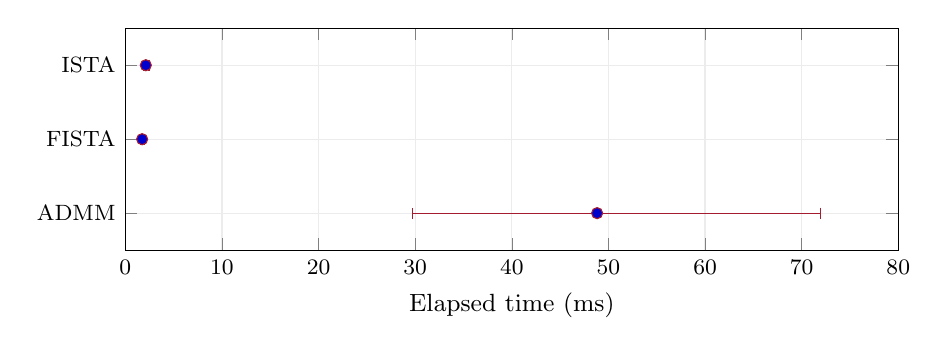
\begin{tikzpicture}
\begin{axis}[width=0.94\linewidth,height=4.4cm,xlabel={Elapsed time (ms)},xmin=0,xmax=80,ytick={1,2,3},yticklabels={ADMM,FISTA,ISTA},ymin=0.5,ymax=3.5]
\addplot+[only marks,mark=*,color=polyured,error bars/.cd,x dir=both,x explicit] coordinates {(2.11784,3) +=(0.33642,0) -=(0.27328,0) (1.73977,2) +=(0.23453,0) -=(0.18397,0) (48.83006,1) +=(23.13594,0) -=(19.12993,0)};
\end{axis}\end{tikzpicture}
\caption{Baseline mean time with 95\% bootstrap intervals. Each point averages twenty within-instance timing medians. The ADMM interval is appreciably wider.}\label{fig:timing}
\end{figure}

To obtain an additive preparation-cost decomposition, we select the complete run with median total time for each seed. The sum of its setup times divided by the sum of its total times is approximately 98\% for baseline ADMM. Selecting setup and total medians independently could select different runs. A workload with repeated right-hand sides could amortize a reused factorization, changing the relative cost.

\subsection{Paired timing comparisons}
FISTA had a lower mean time than ISTA in nine of the ten settings. At baseline, the paired difference, defined as FISTA minus ISTA, was $-0.378$ ms with a 95\% interval of $[-0.637,-0.110]$ ms. Figure~\ref{fig:paired} reports all ten configuration-level paired comparisons.

\begin{figure}[htbp]\centering
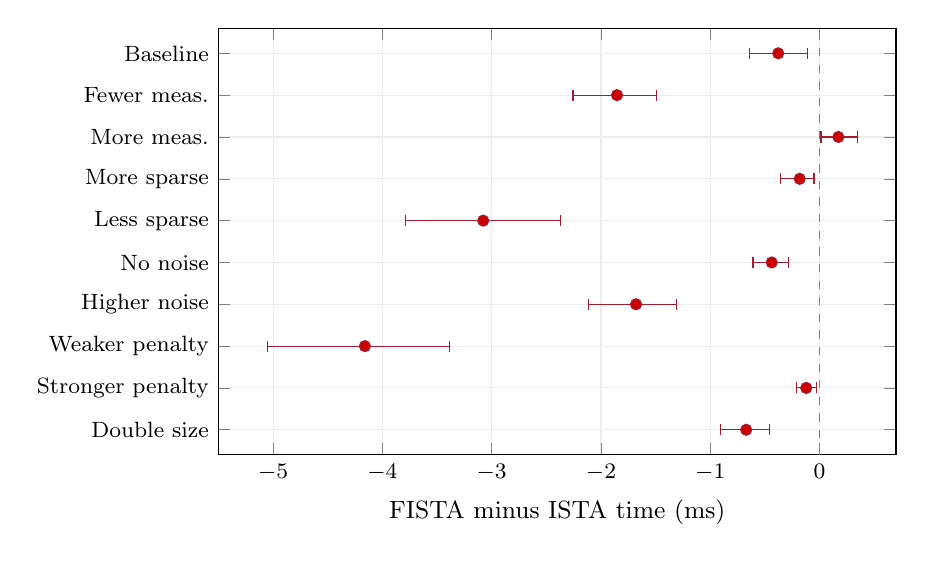
\begin{tikzpicture}
\begin{axis}[width=0.84\linewidth,height=7cm,xlabel={FISTA minus ISTA time (ms)},xmin=-5.5,xmax=0.7,ytick={1,2,3,4,5,6,7,8,9,10},yticklabels={Double size,Stronger penalty,Weaker penalty,Higher noise,No noise,Less sparse,More sparse,More meas.,Fewer meas.,Baseline},ymin=0.4,ymax=10.6]
\addplot[gray,dashed] coordinates {(0,0.4)(0,10.6)};
\addplot+[only marks,mark=*,color=polyured,error bars/.cd,x dir=both,x explicit] coordinates {(-0.37807,10) +=(0.268078751,0) -=(0.258882999,0) (-1.853525,9) +=(0.363624627,0) -=(0.402878877,0) (0.172075001,8) +=(0.178130376,0) -=(0.158472625,0) (-0.181625,7) +=(0.131427247,0) -=(0.175591628,0) (-3.078005,6) +=(0.710430248,0) -=(0.712561875,0) (-0.43739,5) +=(0.154085003,0) -=(0.171036375,0) (-1.67948,4) +=(0.371744875,0) -=(0.432851254,0) (-4.16076,3) +=(0.773274126,0) -=(0.890053501,0) (-0.121845002,2) +=(0.0909207502,0) -=(0.0906251259,0) (-0.671405,1) +=(0.216915249,0) -=(0.232970875,0)};
\end{axis}\end{tikzpicture}
\caption{Paired timing differences across all ten configurations with exploratory 95\% bootstrap intervals. Negative values favor FISTA.}\label{fig:paired}
\end{figure}


With 128 measurements, FISTA averaged 73 iterations and ISTA 91, while FISTA was slower by 0.172 ms, with interval $[0.014,0.350]$ ms. The measurements establish a reversal between iteration and runtime rankings. They do not measure the separate contributions of acceleration updates and other execution overhead. Component-level profiling is required to assign a cause. The strongest selected timing advantage appears with weaker regularization, where FISTA saves about 4.16 ms on average.


\subsection{Convergence trajectories and achieved accuracy}
The baseline trajectory in Figure~\ref{fig:trajectory} reaches the common optimality threshold at 150 updates for ISTA, 100 for FISTA and 40 for ADMM on seed 0. At iteration 20, the respective residuals are 0.05363, 0.02428 and 0.003469. At iteration 30, ADMM is still above the threshold at $1.73\times10^{-4}$, and the next scheduled check records $2.35\times10^{-5}$. This explains the reported endpoint at iteration 40 for that instance. The terminal ISTA and FISTA residuals are $7.46\times10^{-5}$ and $7.34\times10^{-5}$.

The single-instance curve and the configuration averages answer different empirical questions. The curve records the path taken on one draw, whereas the average counts of 148, 95 and 40.5 summarize twenty baseline instances. Across all settings, ADMM has the lowest mean count. In the weakest-penalty setting, mean counts rise to 484.5 for ISTA, 150 for FISTA and 90.5 for ADMM. This condition creates the largest observed iteration ratio between ISTA and FISTA, consistent with the larger runtime advantage recorded there.

\begin{figure}[htbp]\centering
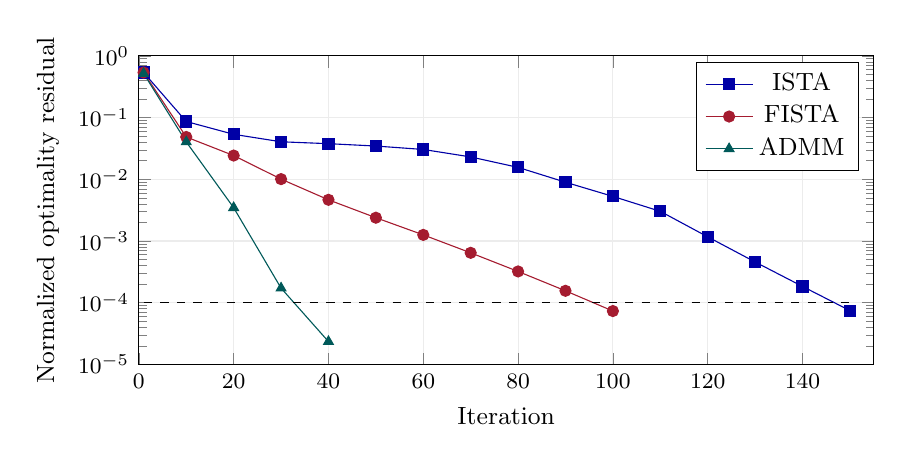
\begin{tikzpicture}
\begin{axis}[width=0.9\linewidth,height=5.5cm,ymode=log,xlabel={Iteration},ylabel={Normalized optimality residual},xmin=0,xmax=155,ymin=1e-5,ymax=1,legend style={at={(0.98,0.98)},anchor=north east}]
\addplot[color=blue!65!black,mark=square*] coordinates {(1,0.538391067) (10,0.0864779378) (20,0.0536305904) (30,0.0405827472) (40,0.037830736) (50,0.0346220482) (60,0.0304816188) (70,0.0230606834) (80,0.015611645) (90,0.00897814847) (100,0.00528851536) (110,0.00303083101) (120,0.00116966503) (130,0.000458006217) (140,0.000183924526) (150,7.46098995e-05)};\addlegendentry{ISTA}
\addplot[color=polyured,mark=*] coordinates {(1,0.538391067) (10,0.0485305423) (20,0.0242790304) (30,0.0100796344) (40,0.00465789622) (50,0.00238714169) (60,0.00125805501) (70,0.000644020873) (80,0.000321479398) (90,0.000156152804) (100,7.33562608e-05)};\addlegendentry{FISTA}
\addplot[color=teal!70!black,mark=triangle*] coordinates {(1,0.519280236) (10,0.0403798199) (20,0.00346949166) (30,0.000172524599) (40,2.34936839e-05)};\addlegendentry{ADMM}
\addplot[black,dashed,forget plot] coordinates {(1,0.0001)(150,0.0001)};
\end{axis}\end{tikzpicture}
\caption{Baseline convergence at seed 0 and repeat label 0. Points are the recorded stopping checks. The dashed line is the shared threshold. The ADMM endpoint also satisfies its feasibility checks.}\label{fig:trajectory}
\end{figure}

\subsection{Iteration reduction and elapsed-time reduction}
Figure~\ref{fig:ratios} compares the reduction in updates with the reduction in measured time. At baseline, the ISTA/FISTA iteration ratio is 1.56, whereas the time ratio is 1.22. Equivalently, FISTA uses 35.8\% fewer updates and 17.9\% less time. With weaker regularization these ratios become 3.23 and 2.56. With 24 nonzeros they are 2.63 and 2.09. Thus the configurations with the largest iteration savings also deliver the largest measured time ratios in this benchmark.

The more-measurements setting produces the clearest divergence. FISTA uses 19.8\% fewer updates, while its mean time is 11.1\% higher. This observation establishes that update count alone does not determine runtime for these implementations. The measurements aggregate gradient calculations, vector operations and convergence checks, so they do not assign the reversal to a specific operation. That attribution requires component-level profiling. The plotted ratios are descriptive ratios of aggregate means, with no ratio confidence intervals inferred from the paired difference intervals.

\begin{figure}[htbp]\centering
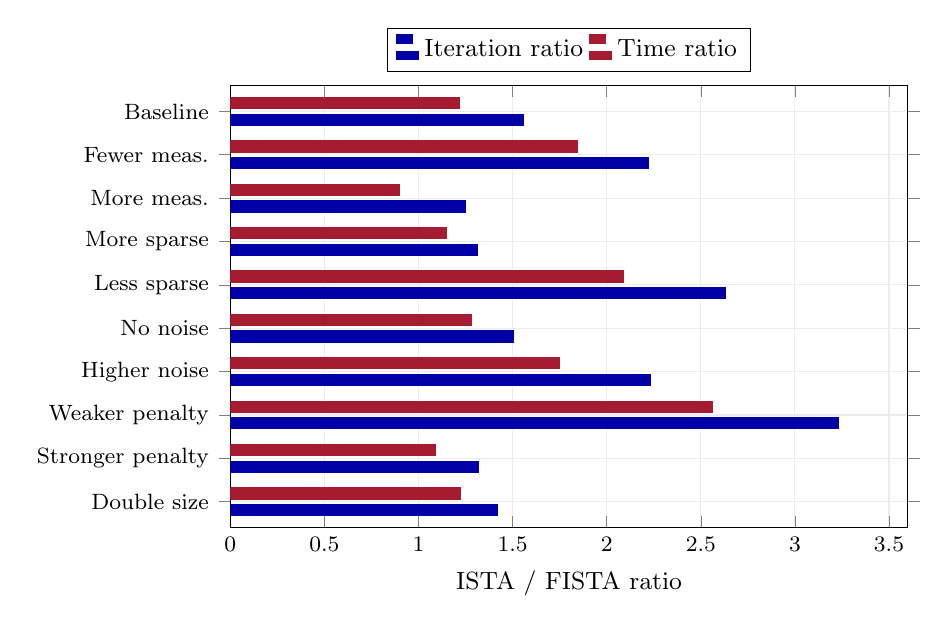
\begin{tikzpicture}
\begin{axis}[width=0.84\linewidth,height=7.2cm,xbar,bar width=4pt,xlabel={ISTA / FISTA ratio},xmin=0,xmax=3.6,ytick={1,2,3,4,5,6,7,8,9,10},yticklabels={Double size,Stronger penalty,Weaker penalty,Higher noise,No noise,Less sparse,More sparse,More meas.,Fewer meas.,Baseline},ymin=0.4,ymax=10.6,legend columns=2,legend style={at={(0.5,1.03)},anchor=south}]
\addplot[fill=blue!65!black,draw=blue!65!black] coordinates {(1.55789474,10) (2.22142857,9) (1.24657534,8) (1.31333333,7) (2.62987013,6) (1.5027933,5) (2.23140496,4) (3.23,3) (1.31818182,2) (1.41798942,1)};\addlegendentry{Iteration ratio}
\addplot[fill=polyured,draw=polyured] coordinates {(1.21731033,10) (1.84318783,9) (0.900126818,8) (1.14607478,7) (2.08758239,6) (1.28135302,5) (1.74826465,4) (2.56066346,3) (1.09233865,2) (1.22233168,1)};\addlegendentry{Time ratio}

\end{axis}\end{tikzpicture}
\caption{Ratios of the mean iteration counts and mean measured times. Values above one favor FISTA. Each ratio compares the archived configuration-level means.}\label{fig:ratios}
\end{figure}

\subsection{ADMM preparation cost across all configurations}
Figure~\ref{fig:setup} shows that the preparation cost dominates every tested configuration under the same-run decomposition. At baseline, preparation accounts for 47.77 ms out of 48.83 ms, leaving 1.06 ms for the remaining measured operations. At double dimensions the corresponding values are 90.13 ms and 1.90 ms. Across the ten settings, the preparation share ranges from 92.33\% under weaker regularization to 97.93\% at double dimensions.

The weaker-penalty case has the largest remaining-time mean, 2.03 ms, together with ADMM's largest mean update count, 90.5. This connects the increased iteration workload to a visible component of elapsed time even while preparation remains dominant. These values use the preparation and total time from the same median-total run. They differ slightly from a decomposition that independently takes medians of each component, because independent medians can select different repetitions.

Removing the measured setup component gives an accounting estimate of time already spent in the remaining operations. It does not measure a redesigned solver. A Cholesky implementation would have its own factorization cost and a different solve cost per update. The present decomposition identifies the dominant measured expense and supplies a concrete target for that follow-up experiment.

\begin{figure}[htbp]\centering
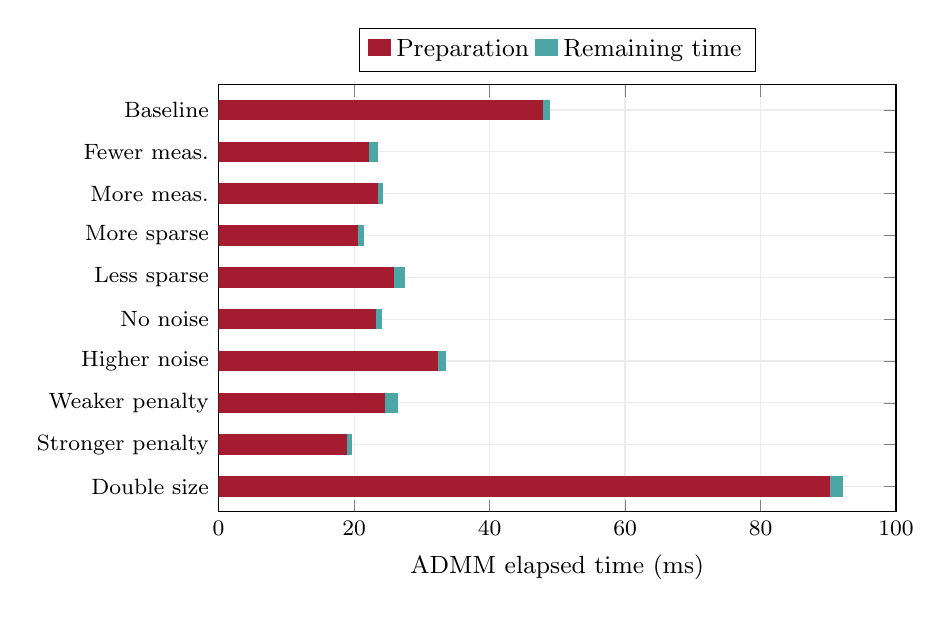
\begin{tikzpicture}
\begin{axis}[width=0.84\linewidth,height=7cm,xbar stacked,bar width=7pt,xlabel={ADMM elapsed time (ms)},xmin=0,xmax=100,ytick={1,2,3,4,5,6,7,8,9,10},yticklabels={Double size,Stronger penalty,Weaker penalty,Higher noise,No noise,Less sparse,More sparse,More meas.,Fewer meas.,Baseline},ymin=0.4,ymax=10.6,legend columns=2,legend style={at={(0.5,1.03)},anchor=south}]
\addplot[fill=polyured,draw=polyured] coordinates {(47.765495,10) (22.08269,9) (23.40521,8) (20.43401,7) (25.780145,6) (23.15794,5) (32.30932,4) (24.420165,3) (18.874925,2) (90.12833,1)};\addlegendentry{Preparation}
\addplot[fill=teal!70,draw=teal!70] coordinates {(1.064565,10) (1.30383499,9) (0.847390002,8) (0.924595003,7) (1.714245,6) (0.842895001,5) (1.16662,4) (2.02788,3) (0.729929999,2) (1.902995,1)};\addlegendentry{Remaining time}
\end{axis}\end{tikzpicture}
\caption{Additive ADMM time decomposition across all configurations. For each seed, preparation and total time come from the same run whose total time is the median of five repeats. Components are then averaged over twenty seeds.}\label{fig:setup}
\end{figure}


\begin{table}[htbp]\centering\small
\caption{ADMM accounting decomposition in milliseconds. Each seed selects the run with median total time; all components use that same run and are then averaged across twenty seeds.}
\begin{tabular}{lrrr}\toprule
Condition & Total & Preparation & Remaining \\\midrule
Baseline & 48.83 & 47.77 & 1.06 \\
Fewer measurements & 23.39 & 22.08 & 1.30 \\
More measurements & 24.25 & 23.41 & 0.85 \\
More sparse & 21.36 & 20.43 & 0.92 \\
Less sparse & 27.49 & 25.78 & 1.71 \\
No noise & 24.00 & 23.16 & 0.84 \\
Higher noise & 33.48 & 32.31 & 1.17 \\
Weaker regularization & 26.45 & 24.42 & 2.03 \\
Stronger regularization & 19.60 & 18.87 & 0.73 \\
Double dimensions & 92.03 & 90.13 & 1.90 \\
\bottomrule\end{tabular}\end{table}
The remaining-time means are below the corresponding ISTA and FISTA total-time means in all ten configurations. This is a descriptive component comparison with unequal timing boundaries. The remaining interval includes initialization, updates and scheduled checks; it is not an isolated update-loop timer or a measurement of a solver that reuses preparation across independent queries. Repeated right-hand-side experiments would be needed to establish the end-to-end benefit of such reuse. We therefore retain total measured time as the primary comparison.

\subsection{Observed timing variability and confidence intervals}
Figure~\ref{fig:variation} examines variability while holding the input instance fixed. For each seed we compute the range of its five times divided by their median. The median of these relative ranges across twenty baseline seeds is 40.4\% for ISTA, 42.4\% for FISTA and 82.4\% for ADMM. The raw timings therefore contain substantial within-instance variability. The larger ADMM variation also appears in its baseline confidence interval, whose width is 42.27 ms, compared with 0.61 ms for ISTA and 0.42 ms for FISTA.

The reported means first reduce each five-repeat group to its median. Pairing then compares solvers on the same input and the bootstrap resamples complete instances. Every FISTA-minus-ISTA interval in the ten-setting archive excludes zero at the unadjusted 95\% level: nine lie below zero and the more-measurements interval lies above zero. This supports the direction of the observed mean differences under the specified analysis. The intervals remain exploratory because ten configuration-level comparisons were examined without multiplicity adjustment, and the original measurements contain one execution environment.

The bootstrap resamples the observed per-instance median estimates. It does not separately fit a model for operating-system delays or estimate performance across different machines. Five repeated timings reduce the influence of isolated slow runs, while Figure~\ref{fig:variation} quantifies the variability that remains in the underlying measurements. Both the effect size and its interval are therefore reported alongside this repeat-level diagnostic.

\begin{figure}[htbp]\centering
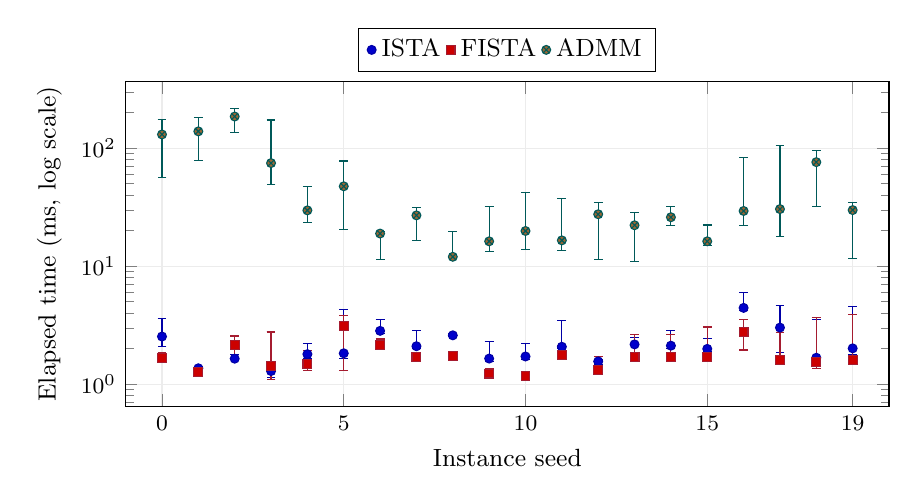
\begin{tikzpicture}
\begin{axis}[width=0.93\linewidth,height=5.7cm,ymode=log,xlabel={Instance seed},ylabel={Elapsed time (ms, log scale)},xmin=-1,xmax=20,xtick={0,5,10,15,19},legend columns=3,legend style={at={(0.5,1.03)},anchor=south}]
\addplot+[only marks,mark size=1.6pt,color=blue!65!black,error bars/.cd,y dir=both,y explicit] coordinates {(0,2.5317) +=(0,1.07120001) -=(0,0.457999995) (1,1.3622) +=(0,0.0492000108) -=(0,0.0153000001) (2,1.643) +=(0,0.143100013) -=(0,0.0326999871) (3,1.2898) +=(0,1.4982) -=(0,0.157899995) (4,1.7944) +=(0,0.429599997) -=(0,0.16190001) (5,1.8254) +=(0,2.4532) -=(0,0.185299999) (6,2.8287) +=(0,0.704699996) -=(0,0.146799997) (7,2.09469999) +=(0,0.749500003) -=(0,0.0979999895) (8,2.592) +=(0,0.0881999877) -=(0,0.0545000075) (9,1.64609999) +=(0,0.654200005) -=(0,0.089299996) (10,1.71490001) +=(0,0.509400008) -=(0,0.102599995) (11,2.073) +=(0,1.4122) -=(0,0.0479999871) (12,1.55830001) +=(0,0.0518999877) -=(0,0.0916999998) (13,2.1708) +=(0,0.29370001) -=(0,0.355900003) (14,2.11700001) +=(0,0.743500001) -=(0,0.127100007) (15,1.98900001) +=(0,0.441700002) -=(0,0.0861000153) (16,4.42919999) +=(0,1.5635) -=(0,0.222899995) (17,3.0139) +=(0,1.6276) -=(0,1.14600001) (18,1.67329999) +=(0,1.8652) -=(0,0.129299995) (19,2.00940001) +=(0,2.51219999) -=(0,0.238599998)};\addlegendentry{ISTA}
\addplot+[only marks,mark size=1.6pt,color=polyured,error bars/.cd,y dir=both,y explicit] coordinates {(0,1.6567) +=(0,0.181099997) -=(0,0.0679999939) (1,1.2634) +=(0,0.0777000096) -=(0,0.0455000118) (2,2.1521) +=(0,0.407399988) -=(0,0.499800008) (3,1.42070001) +=(0,1.34729999) -=(0,0.317900005) (4,1.47240001) +=(0,0.465199992) -=(0,0.163400007) (5,3.1092) +=(0,0.70270001) -=(0,1.81270001) (6,2.15679999) +=(0,0.255699997) -=(0,0.190099992) (7,1.70959999) +=(0,0.0750000036) -=(0,0.0526999938) (8,1.7435) +=(0,0.101700003) -=(0,0.0447000057) (9,1.2282) +=(0,0.130999993) -=(0,0.0350000046) (10,1.1673) +=(0,0.0759000104) -=(0,0.0193000014) (11,1.76079999) +=(0,0.342200001) -=(0,0.0523999915) (12,1.3227) +=(0,0.389699999) -=(0,0.022600012) (13,1.7046) +=(0,0.931300005) -=(0,0.0870000076) (14,1.7005) +=(0,0.952800008) -=(0,0.0394999952) (15,1.7065) +=(0,1.3421) -=(0,0.0815999956) (16,2.76990001) +=(0,0.773299995) -=(0,0.8256) (17,1.603) +=(0,1.14460001) -=(0,0.0911999959) (18,1.54129999) +=(0,2.12030001) -=(0,0.186299992) (19,1.60620001) +=(0,2.28259999) -=(0,0.0758000097)};\addlegendentry{FISTA}
\addplot+[only marks,mark size=1.6pt,color=teal!70!black,error bars/.cd,y dir=both,y explicit] coordinates {(0,130.9363) +=(0,43.288) -=(0,74.1515) (1,139.0471) +=(0,42.1137) -=(0,60.9213) (2,185.8124) +=(0,30.0564) -=(0,48.9361) (3,74.8476) +=(0,98.6939) -=(0,25.8269) (4,29.7385) +=(0,17.7432) -=(0,6.4675) (5,47.5734) +=(0,30.4803) -=(0,27.0216) (6,18.917) +=(0,0.695499984) -=(0,7.44650001) (7,26.9684) +=(0,4.7104) -=(0,10.4518) (8,12.0082) +=(0,7.84889999) -=(0,0.237800006) (9,16.2453) +=(0,15.7331) -=(0,2.84640002) (10,19.8898) +=(0,21.966) -=(0,6.08039999) (11,16.5538) +=(0,20.9839) -=(0,2.9334) (12,27.5635) +=(0,7.273) -=(0,16.2333) (13,22.2284) +=(0,6.52170001) -=(0,11.3013) (14,26.0013) +=(0,5.8074) -=(0,3.73240001) (15,16.2515) +=(0,6.0719) -=(0,1.3933) (16,29.392) +=(0,54.6286) -=(0,7.35020002) (17,30.4832) +=(0,75.2391) -=(0,12.634) (18,76.2515) +=(0,19.3548) -=(0,44.2105) (19,29.892) +=(0,4.49139999) -=(0,18.2363)};\addlegendentry{ADMM}

\end{axis}\end{tikzpicture}
\caption{Within-instance baseline timing variation. Each point is the median of five repeats, and each vertical segment spans their observed minimum and maximum. These segments describe repeated measurements of one fixed instance.}\label{fig:variation}
\end{figure}

\subsection{Measurement conditions and recovery quality}
We use converged FISTA solutions to illustrate recovery, since the final errors of the three solvers are close. Increasing measurements from 64 to 96 reduced mean relative error from 11.57\% to 8.46\%. Increasing to 128 reduced it further to 8.26\%. The second improvement was smaller within this tested range. At five nonzero coefficients the error was 7.08\%, whereas at 24 nonzeros it reached 19.68\%.
\begin{figure}[htbp]\centering
\begin{minipage}{0.49\linewidth}\centering
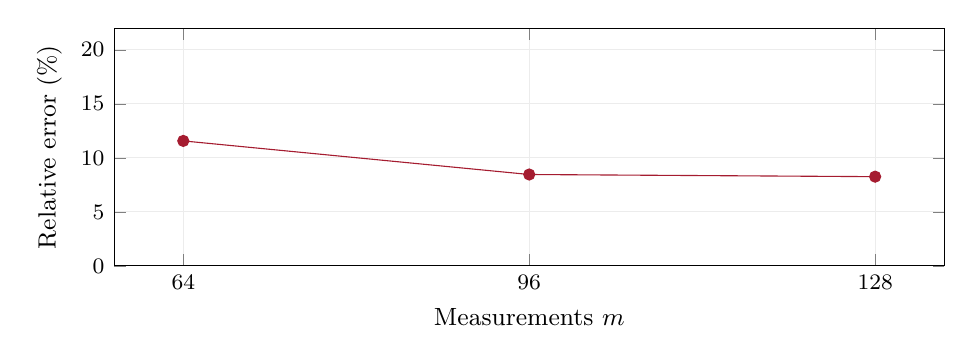
\begin{tikzpicture}\begin{axis}[width=\linewidth,height=4.6cm,xlabel={Measurements $m$},ylabel={Relative error (\%)},xtick={64,96,128},ymin=0,ymax=22]
\addplot[color=polyured,mark=*] coordinates {(64,11.57)(96,8.46)(128,8.26)};
\end{axis}\end{tikzpicture}\end{minipage}\hfill
\begin{minipage}{0.49\linewidth}\centering
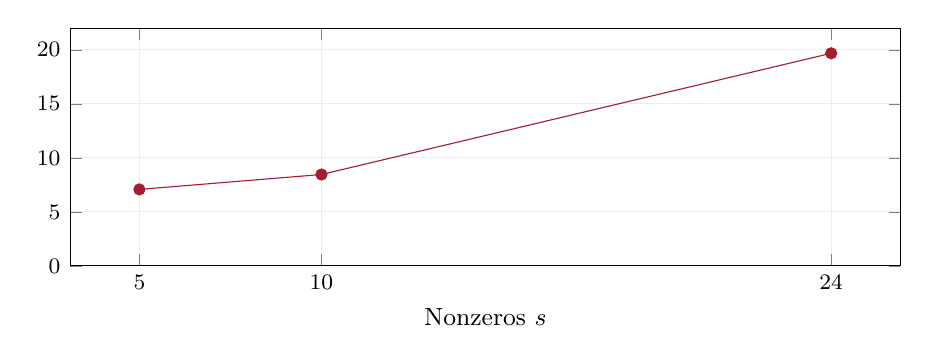
\begin{tikzpicture}\begin{axis}[width=\linewidth,height=4.6cm,xlabel={Nonzeros $s$},xtick={5,10,24},ymin=0,ymax=22]
\addplot[color=polyured,mark=*] coordinates {(5,7.08)(10,8.46)(24,19.68)};
\end{axis}\end{tikzpicture}\end{minipage}
\caption{FISTA mean reconstruction error across measurement and sparsity settings. Lines connect the tested means as visual guides. Each point averages twenty instances.}\label{fig:recovery}
\end{figure}

These comparisons describe changes in the data-generating settings. Changing matrix dimensions can change subsequent random draws, so the same seed across settings need not preserve exactly the same underlying signal. The curves provide evidence within the synthetic distribution and range tested.


The measurement-count sweep provides a quantitative comparison of marginal improvements. Adding 32 measurements to the 64-measurement setting reduces error by 3.11 percentage points, or 26.9\% relative to that setting. Adding a further 32 measurements reduces error by 0.20 percentage points, or 2.4\% relative to baseline. In the sparsity sweep, increasing the active count from 5 to 24 multiplies mean error by 2.78. Both statements refer to the empirical means in the tested range. They establish the magnitude of the observed changes without identifying a universal measurement threshold.

At fixed $m=96$ and $n=192$, increasing the active count from 10 to 24 raises FISTA's mean iteration count from 95 to 154 and mean time from 1.74 to 2.83 ms. The same perturbation also raises its reconstruction error from 8.46\% to 19.68\%. In this comparison, the less-sparse problem is harder in both computational and recovery terms. The distinction remains necessary because the penalty sweep below moves computation and recovery in opposite directions.

\subsection{Regularization, noise and scale}
On baseline data, increasing $\alpha$ from 0.01 to 0.05 to 0.15 reduced FISTA time from 2.67 to 1.74 to 1.32 ms. Reconstruction error increased from 5.26\% to 8.46\% to 24.43\%. Figure~\ref{fig:tradeoff} combines these two outcomes. Stronger shrinkage introduces bias, and the fastest setting in this sweep also has the largest reconstruction error.
\begin{figure}[htbp]\centering
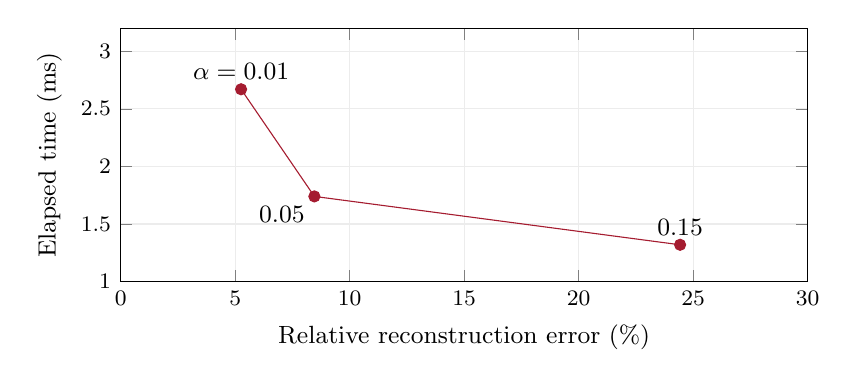
\begin{tikzpicture}\begin{axis}[width=0.85\linewidth,height=4.8cm,xlabel={Relative reconstruction error (\%)},ylabel={Elapsed time (ms)},xmin=0,xmax=30,ymin=1,ymax=3.2]
\addplot[color=polyured,mark=*] coordinates {(5.26,2.67)(8.46,1.74)(24.43,1.32)};
\node[anchor=south] at (axis cs:5.26,2.67) {$\alpha=0.01$};
\node[anchor=north east] at (axis cs:8.46,1.74) {$0.05$};
\node[anchor=south] at (axis cs:24.43,1.32) {$0.15$};
\end{axis}\end{tikzpicture}
\caption{Time and recovery error for three regularization strengths on baseline data. Both coordinates are means over twenty instances. No validation set was used to select $\alpha$.}\label{fig:tradeoff}
\end{figure}

With zero measurement noise, baseline regularization still leaves 8.22\% mean error. Increasing the noise standard deviation to 0.08 raises mean error to 20.10\%. Since $\lambda$ depends on $b$, the noise sweep also allows the regularization weight to change. Fixing $\lambda$ across noise levels would isolate a different experimental question. Doubling $m,n,s$ raises mean ADMM time to 92.03 ms and FISTA time to 3.02 ms. Two sizes provide a limited scaling comparison.


Between $\alpha=0.01$ and $\alpha=0.15$, the reported FISTA time decreases by 50.6\%, while error increases by 19.17 percentage points and becomes 4.64 times as large. The three points therefore form a measured time--error trade-off. Selecting the fastest point would select the largest error among the three tested settings. A selection rule based on an external accuracy target or held-out data is needed to choose the penalty for an application.

For an active coefficient at an optimum, the LASSO first-order condition has the form $[A^\top(A\widehat x-b)]_j=-\lambda\operatorname{sign}(\widehat x_j)$. The penalty therefore balances a nonzero fitting gradient against shrinkage on active coordinates. This explains why a nonzero penalty can retain bias even when measurement noise is zero. The observed zero-noise error of 8.22\% is consistent with this mechanism. The experiment does not decompose that error into separate contributions from regularization and the inverse problem.

When the noise standard deviation increases fourfold, from 0.02 to 0.08, error rises from 8.46\% to 20.10\%, a 137.6\% relative increase. This is the outcome of the full stated reconstruction procedure, including the data-dependent rule for $\lambda$. In the size experiment, FISTA's mean count stays almost constant, from 95 to 94.5, while time rises by a factor of 1.74. The matrices have four times as many entries. The measured time ratio therefore captures this particular dense-library and problem-size regime, and two size points do not identify an empirical complexity exponent.

\begin{table}[htbp]\centering
\caption{Complete shared-study results. Times are means of within-instance medians, in milliseconds. Recovery error is the FISTA mean, in percent.}\label{tab:results}
\small\begin{tabular}{lrrrr}\toprule
Condition & ISTA & FISTA & ADMM & Error (\%)\\\midrule
Baseline &2.12&1.74&48.83&8.46\\
Fewer measurements &4.05&2.20&23.39&11.57\\
More measurements &1.55&1.72&24.25&8.26\\
More sparse &1.42&1.24&21.36&7.08\\
Less sparse &5.91&2.83&27.49&19.68\\
No noise &1.99&1.55&24.00&8.22\\
Higher noise &3.92&2.24&33.48&20.10\\
Weaker regularization &6.83&2.67&26.45&5.26\\
Stronger regularization &1.44&1.32&19.60&24.43\\
Double dimensions &3.69&3.02&92.03&9.78\\\bottomrule
\end{tabular}\end{table}

\FloatBarrier
\section{Reproducibility and limitations}
The accompanying repository contains the NumPy solver implementations, the pilot study of 180 runs, the main 3,000-run archive, per-instance medians, bootstrap summaries, paired comparisons and convergence traces. The main experiment is generated by \texttt{extended\_experiments.py}. A verification script reconstructs the grouped medians, summary means and bootstrap intervals from individual runs. Re-execution during repository preparation reproduced all archived iteration counts, with objective differences below $10^{-9}$. New timings depend on the local execution environment.

The historical software environment and seeds are recorded, but hardware details and thread settings were not fully captured. The benchmark uses small, column-normalized Gaussian matrices, a fixed ADMM penalty and an explicit inverse implementation. Timing boundaries and stopping checks differ across solvers. Repeated timings and random ordering reduce measurement variability, while cross-machine replication would be needed to assess hardware generality.

The separate 2,000-run supplementary experiment in the FISTA presentation is outside the shared evidence used here. Its full source and per-run records were not available in the assembled materials. All three-way comparisons in this report use the archived shared study.

\section{Conclusions}
The three solvers reached their specified thresholds in all 3,000 runs, with a maximum within-instance objective spread of $2.30\times10^{-6}$. FISTA reduced mean time in nine of ten configurations. Its baseline reduction was 17.9\%, increasing to 60.9\% under weaker regularization. ADMM achieved the lowest mean iteration count in every configuration, while preparation consumed 92.33--97.93\% of its measured total time under the same-run decomposition. Across the three baseline penalty values, increasing $\alpha$ from 0.01 to 0.15 cut FISTA time by 50.6\% and raised recovery error from 5.26\% to 24.43\%.

The next useful comparisons are a paired evaluation of factorized ADMM solves, separate accounting of cold and reused preparation, and a noise sweep with fixed $\lambda$. Structured matrices, real signals and larger problems would extend the range of evidence. The present results support reporting objective accuracy, recovery error, iteration count and elapsed time together.

\begin{thebibliography}{9}
\bibitem[Beck and Teboulle(2009)]{beck2009}
Amir Beck and Marc Teboulle. A fast iterative shrinkage-thresholding algorithm for linear inverse problems. \emph{SIAM Journal on Imaging Sciences}, 2(1):183--202, 2009. \url{https://doi.org/10.1137/080716542}.
\bibitem[Boyd and Vandenberghe(2004)]{boyd2004}
Stephen Boyd and Lieven Vandenberghe. \emph{Convex Optimization}. Cambridge University Press, 2004. \url{https://web.stanford.edu/~boyd/cvxbook/}.
\bibitem[Boyd et al.(2011)]{boyd2011}
Stephen Boyd, Neal Parikh, Eric Chu, Borja Peleato and Jonathan Eckstein. Distributed optimization and statistical learning via the alternating direction method of multipliers. \emph{Foundations and Trends in Machine Learning}, 3(1):1--122, 2011. \url{https://web.stanford.edu/~boyd/papers/admm_distr_stats.html}.

\bibitem[Tibshirani(1996)]{tibshirani1996}
Robert Tibshirani. Regression shrinkage and selection via the lasso. \emph{Journal of the Royal Statistical Society: Series B}, 58(1):267--288, 1996. \url{https://doi.org/10.1111/j.2517-6161.1996.tb02080.x}.
\bibitem[Parikh and Boyd(2014)]{parikh2014}
Neal Parikh and Stephen Boyd. Proximal algorithms. \emph{Foundations and Trends in Optimization}, 1(3):123--231, 2014. \url{https://web.stanford.edu/~boyd/papers/prox_algs.html}.
\bibitem[Tibshirani(2013)]{tibshirani2013}
Ryan J. Tibshirani. The lasso problem and uniqueness. \emph{Electronic Journal of Statistics}, 7:1456--1490, 2013. \url{https://www.stat.cmu.edu/~ryantibs/papers/lassounique.pdf}.
\end{thebibliography}
\end{document}
